\chapter{Brückenkapitel (0)}
In ersten Kapitel, oder eher im nullten gemäss Aufgabenbuch, repetieren wir einige Dinge, die ihr auf der Oberstufe gelernt habt. Damit sind wir dann alle auf dem gleichen Stand, und teilweise erweitern wir unser Wissen bereits etwas, führen vielleicht neue Schreibweisen ein, formulieren die Rechengesetze evtl. etwas allgemeiner oder manchmal abstrakter, als du es bisher gewohnt warst. Vielleicht ist das für dich zum grössten Teil ein alter Hut - aber Übung macht den Meister!

\section{Die Rechengesetze}
Ein Gesetz ist bekanntermaßen eine feste Regel oder eine verbindliche Vorschrift. An ihm darf man nichts rütteln oder verschieben, sondern man muss sich daran halten. Genauso, wie es in den Gesetzbüchern Gesetze gibt, gibt es auch in der Mathematik Regeln, die gelten und beim Rechnen eingehalten werden müssen. Diese sind die Rechengesetze oder Rechenregeln.

\begin{tcolorbox}[colback=green!10!white,colframe=green!70!black,title=Rechengesetz,width=.9\linewidth]
		Ein Rechengesetz ist eine verbindliche Rechenvorschrift.
\end{tcolorbox}

Wenn du ein Rechengesetz missachtest, bekommst du natürlich keine Strafe von der Polizei. Du wirst aber mit Sicherheit Punkte in deiner Klausur verlieren. Denn: wenn du dich an die Rechengesetze nicht hältst, dann wird auch dein Ergebnis falsch sein. Die Rechengesetze gibt es also nicht, um verzweifelte SchülerInnen zu quälen, sondern sie ergeben mathematisch und logisch Sinn.

Wenn man von den Rechengesetzen spricht, dann meint man meistens das Assoziativgesetz, das Kommutativgesetz und das Distributivgesetz. Sie sind die drei wichtigsten Rechengesetze.Wenn man den Begriff aber etwas weiter fasst, gibt es noch einige weitere Rechenregeln. Diese sind etwa die Regel Punkt-vor-Strich, die Potenzgesetze und die Wurzelgesetze, oder Vorgehensweisen zum Auflösen von Klammern. Fangen wir also an.

\subsection{Rechengesetze}

\begin{tcolorbox}[colback=red!10!white,colframe=red!70!black,title=Rechengesetze,width=.9\linewidth]
	\begin{enumerate}
		\item
			Punktrechnungen ( $\cdot$ und : ) müssen vor Strichrechnungen ( + und - ) ausgeführt werden.
		\item
			Klammern in Termen müssen zuerst aufgelöst werden. ("`von innen nach aussen"')
		\item
			Kommen Potenzen vor, müssen diese als erstes berechnet werden.
		\item
			Assoziativgesetz der Addition: Für alle rellen Zahlen $a$, $b$ und $c$ gilt: $(a+b)+c = a+(b+c)$
		\item
			Assoziativgesetz der Multiplikation: Für alle rellen Zahlen $a$, $b$ und $c$ gilt: $(a\cdot b)\cdot c = a\cdot (b\cdot c)$
		\item
			Kommutativgesetz der Addition: Für alle rellen Zahlen $a$ und $b$ gilt: $a+ b= b+ a$
		\item
			Kommutativgesetz der Multiplikation: Für alle rellen Zahlen $a$ und $b$ gilt:$a\cdot b= b\cdot a$
		\item
			Distributivgesetz der Multiplikation: Für alle rellen Zahlen $a$, $b$ und $c$ gilt: $(a\pm b)\cdot c = a\cdot c \pm b\cdot c$
		\item
			Distributivgesetz der Division: Für alle rellen Zahlen $a$, $b$ und $c$ gilt: $(a\pm b): c = a: c \pm b: c$	
	\end{enumerate}
		
\end{tcolorbox}

\begin{example}
Im folgenden Term darf nicht einfach von links nach rechts gerechnet werden, sondern es muss zuerst das Produkt berechnet werden:
\[
	5+5\cdot 3
\]
\end{example}

\begin{example}
Berechne den folgenden Term:
\[
	4\cdot(27-(3\cdot (5+3)+2))
\]
\end{example}

\begin{example}
Rechne vorteilhaft:
\[
	85+33+67
\]
\end{example}

\begin{example}
Rechne vorteilhaft:
\[
	7\cdot 4 \cdot 45
\]
\end{example}

\begin{example}
Ebenso:
\[
	24+33+76
\]
\end{example}

\begin{example}
Multipliziere aus:
\[
	4\cdot (20-5)
\]
\end{example}

\begin{example}
Manchmal bringt ausklammern einen Vorteil!
\[
	14\cdot 13 - 4\cdot 13
\]
\end{example}

\begin{tcolorbox}[colback=green!10!white,colframe=green!70!black,title=Betrag einer Zahl,width=.9\linewidth]
		Für eine Zahl $a$ ist der Betrag der Zahl
		\[
			|a|=\left\{\begin{array}{ll} a, & a\ge 0 \\
         -a, & a<0\end{array}\right.
		\]
\end{tcolorbox}


\section{Terme}
\subsection*{Auswerten}
Mit $T(a,b)$ bezeichnen wir einen Term, der die Variablen $a$ und $b$ enthält. Setzt man anstelle von $a$ und $b$ Zahlen ein, z.B. 5 für $a$ und 3 für $b$, so schreiben wir $T(5,3)$.
\vspace{1cm}

\subsection*{Termumformungen}
Zwei Terme $T_1$ und $T_2$ heissen \emph{äquivalent (gleichwertig)}, wenn alle möglichen Einsetzungen für die Variable(n) bei $T_1$ denselben Wert ergeben wie bei $T_2$. Man schreibt: $T_1 = T_2$.
\vspace{5mm}
Einen Term umformen bedeutet: Man ersetzt ihn durch einen äquivalenten Term. Beim Umformen von Termen werden die arithmetischen Grundgesetze gebraucht.

\begin{tcolorbox}[colback=red!7!white,colframe=red!60!black,title=Arithmetische Grundgesetze]
	\begin{tabularx}{\linewidth}{|X|c|c|}
			\hline
			 & Addition & Multiplikation \\
			\hline
			Kommutativgesetz & $a+b=b+a$ & $a\cdot b = b\cdot a$ \\
			
			Assoziativgesetz & $(a+b)+c = a+ (b+c)$ & $(a\cdot b)\cdot c = a\cdot (b\cdot c)$ \\
			
			Neutralelement 0 bzw. 1 & $a+0 = a$ & $a\cdot 1 = a$ \\
			
			Inverses Element $-a$ bzw. $\displaystyle \frac{1}{a}$ & $a+(-a) = 0$ & $\displaystyle a\cdot \frac{1}{a} = 1$ \\
			\hline
			Distributivgesetz & \multicolumn{2}{|c|}{$a(b+c)=ab+ac$} \\
			\hline
		\end{tabularx}
		\label{law:arithmetic}
\end{tcolorbox}

\subsection*{Formeln}
Die \emph{Binomischen Formeln} benutzt man zum schnellen Umformen von Produkten aus Binomen. Sie stellen Merkformeln dar, die einerseits das Ausmultiplizieren von Klammerausdrücken erleichtern, andererseits aber auch die Faktorisierung von Termen (Umformung von bestimmten Summen und Differenzen in Produkte) erlauben.

\begin{tcolorbox}[colback=blue!7!white,colframe=blue!60!black,title=Binomische Formeln]
	\begin{tabbing}
		$(a+b)^2$ \qquad \, \, \= $=$ \, \= $a^2+2ab+b^2$ \\
		$(a-b)^2$ \qquad \, \, \= $=$ \, \= $a^2-2ab+b^2$ \\
		$(a+b)(a-b)$ \> $=$ \> $a^2-b^2$
	\end{tabbing}
\end{tcolorbox} 

Es gibt auch trinomische Formeln: $(a+b+c)^2$. Kannst du dafür auch einen Ausdruck angeben?
\vspace{2cm}

\subsection*{Erweiterung}
Mit dem \emph{Pascalschen Dreieck} kann man auch höhere Potenzen von Binomen schnell ausmultiplizieren:
\[
	(a+b)^3 =
\]


\newpage

\section{Im Reich der Zahlen}
\subsection{Natürliche Zahlen}
Die natürlichen Zahlen 1, 2, 3, 4, \ldots ~sind die ältesten Zahlen, die sich aus dem Zählen von Gegenständen entwickelt haben.
Dabei nimmt man an, dass man immer weiterzählen kann.\\

\begin{defn}{Natürliche Zahlen}
	Die Menge der natürlichen Zahlen wird mit $\N$ bezeichnet.
	Man schreibt:
	\begin{align*} 
	 \N = \{ 1, 2, 3, 4, \ldots \}\, .
	\end{align*}
	Die Zahlen $1, 2, 3, 4, \ldots$ heissen \emph{Elemente} der Menge $\N$.
	Ist eine Zahl $n$ eine natürliche Zahl, so schreibt man: $n\in\N$\,.
\end{defn}

\vspace{.5cm}
\begin{wrapfigure}{r}{6cm}
	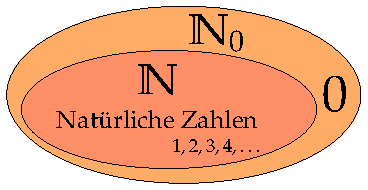
\includegraphics[width=\linewidth]{numberset-naturals-N0}
\end{wrapfigure}
Das Zeichen \glqq $\in$\grqq~bedeutet: \glqq ist Element von\grqq, das Zeichen \glqq $\notin$\grqq~bedeutet: \glqq ist \emph{nicht} Element von\grqq.

\paragraph{Achtung!}
Die Zahl 0 wird dabei {\bfseries nicht} mit dazu genommen.
Wir schreiben:
\begin{align*}
  0 \notin \N\, .
\end{align*}
Möchte man die Null mit einschliessen, so verwenden wir die Schreibweise $\N_0$.\\

\begin{defn}{Natürliche Zahlen zusammen mit Null}
	Die Menge der natürlichen Zahlen wird mit $\N_0$ bezeichnet.
	Man schreibt: $\N_0 = \{ 0, 1, 2, 3, 4, \ldots \}$\,.
\end{defn}

\begin{example}
  Schreibe in das Symbol \relationBox das richtige Zeichen $\in$ oder $\notin$ hinein.
  \begin{align*}
   2 \relationBox \N_0\,,\qquad
   \frac{1}{2} \relationBox \N\,,\qquad
   0 \relationBox \N\,,\qquad
   0 \relationBox \N_0\,,\qquad
   \frac{72}{36} \relationBox \N\,.
  \end{align*}

\end{example}


\vspace{.5cm}
Die natürlichen Zahlen braucht man z.B. um Anzahlen anzugeben, Rangplätze oder Reihenfolgen festzulegen oder (bestimmte) Messergebnisse festzuhalten.

\begin{example}~
	\begin{itemize}\setlength\itemsep{0pt}
		\item Wir haben heute 6 Lektionen. (Anzahl)
		\item Heute ist der erste Tag des Monats. (Rangplatz)
		\item Heute ist es 30 Grad warm. (Messergebnis)
	\end{itemize}
\end{example}

Man kann mit den natürlichen Zahlen auch (bestimmte) Gleichungen lösen.
\begin{example}
 Heute ist es \unit[30]{°C} warm und damit \unit[2]{°C} wärmer als gestern.
 D.h. für die Temperatur $x$ von gestern in \unit{°C} gilt die Gleichung:
 \begin{align*}
   x + 2 = 30
 \end{align*}
Die Lösung der Gleichung ist eine natürliche Zahl, nämlich $x = 28$\,, d.h. die gesuchte Temperatur ist \unit[28]{°C}
\end{example}


\subsection{Negative ganze Zahlen}
\begin{wrapfigure}{r}[1cm]{5cm}
 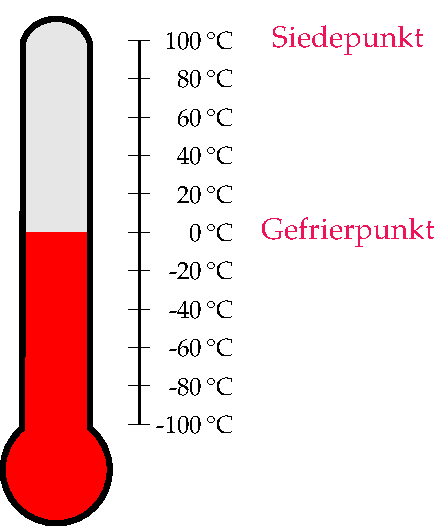
\includegraphics[width=\linewidth]{thermometer}
\end{wrapfigure}
Für viele Zwecke reichen die natürlichen Zahlen nicht aus.
Ist es heute z.B. \unit[30]{°C} warm und wir wollen es mit der Temperatur vor einem halben Jahr vergleichen, so stellen wir vielleicht fest, dass es heute \unit[35]{°C} wärmer ist als vor einem halben Jahr.
D.h. die Temperatur $x$ vor einem halben Jahr in \unit{°C} erfüllt die Gleichung:
\begin{align*}
	x + 35 = 30
\end{align*}
Diese Gleichung lässt sich nicht mit den natürlichen Zahlen lösen, wohl aber, wenn wir negative Zahlen zulassen.
Dann erhalten wir: $x = -5$\,, d.h. die Temperatur ist \unit[--5]{°C}\,.

\subsubsection{Weitere Beispiele}
Die folgenden Beispiele zeigen, dass im Alltag negative Zahlen oft in Verbindung mit einer künstlich festgelegten Null vorkommen.

\paragraph{Temperatur.}
In Europa misst man die Temperatur in \unit{°C}.
Diese Temperaturskala ist so definiert, dass bei Normaldruck der Gefrierpunkt des Wasser gleich \unit[0]{°C} entspricht und der Siedepunkt gleich \unit[100]{°C}.
Wenn eine Temperatur also unter der Temperatur des Wassergefrierpunkts ist, so ist sie negativ.

\paragraph{Meter über dem Meeresspiegel.}
Auf Landkarten wird die Höhe z.B. in Metern über dem Meeresspiegel (m ü.M.) angegeben.
Zum Beispiel liegt der Gipfel des Mt. Whitney in den USA \unit[4418]{m} über dem Meer, kurz \unit[4418]{m ü.M.}
Dabei wurde der Meeresspiegel künstlich als \emph{Normalhöhe} festgelegt.
Dies führt dazu, dass das sogenannte \emph{Tal des Todes} sich bei \unit[-86]{m ü.M.} befindet.

\subsubsection{Zahlengerade}
\begin{figure}[H]
	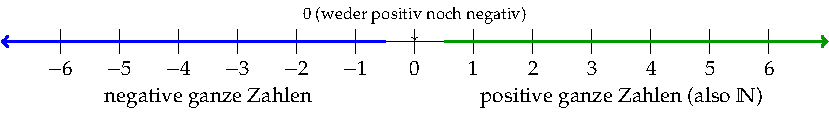
\includegraphics[width=\linewidth]{zahlengerade}
	\caption{Die Zahlengerade mit den positiven ganzen Zahlen rechts von der Null und den negativen ganzen Zahlen links von der Null.
	Die Null ist weder positiv noch negativ.}
	\label{fig:zahlengerade-pos-neg}
\end{figure}

Die sogenannten negativen ganzen Zahlen $-1, -2, -3, \ldots$ stehen links von 0 auf der Zahlengeraden, siehe Abbildung \ref{fig:zahlengerade-pos-neg}.
Die natürlichen Zahlen, die auch positive ganze Zahlen genannt werden, stehen rechts von Null auf der Zahlengeraden. Beachte, dass die Null selbst weder positiv noch negativ ist.
Möchtest du die Zahlen in $\N_0$ auf diese Weise bezeichnen (also die Null mit einschliessen), so kannst du sie nicht-negative ganze Zahlen nennen.

\subsection{Ganze Zahlen}
\begin{wrapfigure}{r}{7cm}
	\vspace{-1cm}
	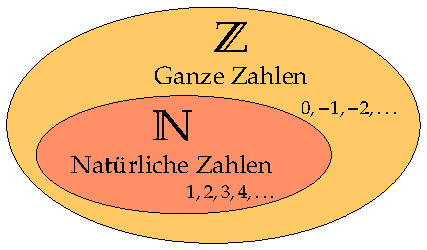
\includegraphics[width=\linewidth]{numberset-integers}
	% \caption{Die natürlichen Zahlen sind in den ganzen Zahlen enthalten.
	% Auf eine Darstellung der Menge $\N_0$ wurde hier für die bessere Übersicht verzichtet.}
	% \label{fig:numberset-integers}
	\vspace{-2cm}
\end{wrapfigure}
Die Menge der ganzen Zahlen besteht aus den natürlichen Zahlen, den negativen ganzen Zahlen und der Null.

Jede natürliche Zahl ist auch eine ganze Zahl, aber nicht andersherum.
D.h. die Menge der natürlichen Zahlen ist komplett in der Menge der ganzen Zahlen enthalten.
%, siehe Abbildung \ref{fig:numberset-integers}.

\vspace{1cm}
\begin{defn}{Ganzen Zahlen}
	Fügt man zu den natürlichen Zahlen $\N$ die Zahl 0 und die negativen ganzen Zahlen $-1, -2, -3,\ldots$ hinzu,
	so erhält man die Menge der ganzen Zahlen $\Z = \{ \ldots, -3, -2, -1, 0, 1, 2, 3, \ldots \}$\, .
\end{defn}


\subsubsection{Regeln}
Für das Rechnen mit den ganzen Zahlen gelten die arithmetischen Grundgesetze, bis auf eine Ausnahme!
Welche? (Schreibe es selber auf.)\\
\kariert{15}{2}\\~\\
Vervollständige die Übersicht von Seite \pageref{law:arithmetic} für alle Regeln bis auf die, die nicht gilt:
\begin{law}{Arithmetische Grundgesetze für \underline{\bfseries die ganzen Zahlen}}
    \bgroup
    \def\arraystretch{2.5}
	\begin{tabularx}{\linewidth}{|X|p{3.7cm}|p{3.7cm}|}
			\hline
			 & Addition & Multiplikation \\
			\hline
			Kommutativgesetz &  &  \\\hline
			Assoziativgesetz &  &  \\\hline
			Es gibt Neutralelement\newline 0 bzw. 1\,. &  &  \\\hline
			Es gibt inverses Element\newline~ & & \\
			\hline
			Distributivgesetz & \multicolumn{2}{c|}{} \\
			\hline
    \end{tabularx}
    \egroup
\end{law}

\subsubsection{Subtraktion}
Mithilfe der negativen Zahlen kann man die Subtraktion als eine Addition mit einer negativen Zahl schreiben. Dabei gelten die arithmetischen Rechenregeln.
\begin{example} Kommutativgesetz der Addition:
	\begin{align*}
					8 - 5		&\,=\, 8 + (-5) \,=\, (-5) + 8\\
		\text{Aber:}\quad 8 - 5		&\,\neq\, 5 - 8
	\end{align*}
	Wende das Kommutativgesetz einmal nach dem gleichen Schema selbst an:\\
	\kariert[\large 10 -- 3 \,=\,]{15}{1.5}\\
\end{example}
\begin{example} Assoziativgesetz der Addition:
	\begin{align*}
					(8 - 5) - 1			&\,=\, \bigl(8 + (-5)\bigr) + (-1) \,=\, 8 + \bigl( (-5) + (-1)\bigr)\\
		\text{Aber:}\quad (8 - 5) - 1	&\,\neq\, 8 - (5 - 1)
	\end{align*}
	Wende das Assoziativgesetz einmal nach dem gleichen Schema selbst an:\\
	\kariert[\large (10 -- 3) -- 2 \,=\,]{15}{2}\\
\end{example}
\begin{example} $(-1)$ ausklammern:
	\begin{align*}
					1 -(8 - 5)			&\,=\, 1 + (-1)\cdot\bigl(8 + (-5)\bigr)\,=\, 1 + (-1)\cdot 8 + (-1)\cdot (-5) = 1 - 8 + 5\\
	\end{align*}
	Klammere $(-1)$ aus:\\
	\kariert[\large 10 -- (3 -- 2) \,=\,]{15}{2}\\
\end{example}

\subsection{Rationale Zahlen}
\begin{wrapfigure}{r}[1cm]{7cm}
	\vspace{-2cm}
	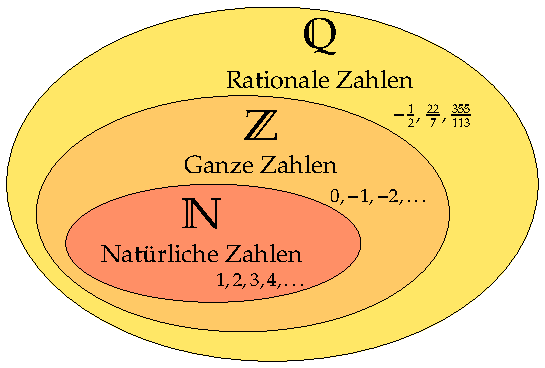
\includegraphics[width=\linewidth]{numberset-rational}
	\vspace{-2cm}
\end{wrapfigure}
In den arithmetischen Grundgesetzen für die ganzen Zahlen sehen wir, dass wir uns das inverse Element für die Multiplikation fehlt.
Führen wir dies ein, so erhalten wir die Menge der rationalen Zahlen $\Q$, die alle Zahlen enthält, die man als Bruch darstellen kann. 
\newpage
\begin{defn}{Rationale Zahlen}
	Die Menge der rationalen Zahlen $\Q$ besteht aus allen Zahlen, die man als Bruch schreiben kann.
	\begin{align*}
		\Q = \left\{\left. \frac{p}{q} ~\right|~ p,q \in \Z;~ q \neq 0\, \right\}
	\end{align*}
\end{defn}

~\\~\\
In dieser Menge können wir schon relativ viel machen.
Jedoch stellen wir fest, dass wir z.B. die Gleichung $x^2 = 2$ nicht über den rationalen Zahlen lösen können.

\begin{claim}
 Man kann $\sqrt{2}$ nicht als Bruch darstellen.
\end{claim}

\begin{proof}
 Schreibe hier den Beweis nochmal für dich selbst auf.
 \vfill
\end{proof}

\newpage
\subsubsection{Abbrechende und periodische Dezimalzahlen}
\label{sec:periodic}

~\vspace{.5cm}
\begin{law}{Brüche sind entweder abbrechende oder periodische Dezimalzahlen.}
\label{law:rationalsArePeriodic}
	In der Dezimaldarstellung ist eine rationale Zahl entweder ein abbrechende Dezimalzahl oder eine periodische.
\end{law}
~
\begin{example}~
	\begin{enumerate}[a)]
		\setlength\itemsep{0pt}
		\item $\frac{1}{50} = 0.02$
		\item $\frac{7}{40} = 0.175$
		\item $\frac{2}{3} = 0.\overline{6}$
		\item $\frac{1}{7} = 0.\overline{142857}$
	\end{enumerate}
\end{example}

Angenommen, eine Zahl ist in der Dezimaldarstellung eine abbrechende Dezimalzahl.
Begründe anhand eines Beispiels, warum es dann möglich ist, den Nenner in der Form 10 oder 100 oder 1000 oder 10\,000 \ldots darzustellen:\\~\\
\kariert{15}{4}\\

Begründe, warum es deshalb für eine abbrechende Dezimaldarstellung notwendig ist, dass der Nenner der Zahl keine Primteiler abweichend von 2 und 5 enthält:\\~\\
\kariert{15}{4}

\newpage
\begin{xmpl}
	Hier sind zwei Beispiele für periodische Dezimalzahlen. Berechne die Dezimaldarstellung mithilfe der schriftlichen Division:\\
 
	\kariertTop[$3~~~:~~~7~=$]{14.5}{8}\\~\\
	\kariertTop[$6~~~:~~~1~~~1~=$]{14.5}{6}\\
\end{xmpl}

Begründe in eigenen Worten, warum Brüche in der Dezimaldarstellung entweder abbrechen oder periodisch werden.\\
\kariert{14.5}{3}

Jetzt wissen wir, wie wir vom Bruch zum Dezimalbruch kommen.%
\footnote{\begin{minipage}[t]{.85\linewidth}
			Quelle: \url{https://www.kapiert.de/mathematik/klasse-5-6/dezimalbrueche/}\\\url{periodische-dezimalbrueche-und-anwendungsaufgaben/}\\
			\url{periodische-dezimalbrueche-in-brueche-umwandeln/}, abgerufen am 03.09.2024.
		\end{minipage}
		\hfill
		\begin{minipage}[t]{.1\linewidth}
			~\\\vspace{-.8cm}
			
\includegraphics[width=\linewidth]{figures/QR-periodischeBrueche}
		\end{minipage}}
Aber schaffen wir es auch, aus einem periodischen Dezimalbruch den zugehörigen gewöhnlichen Bruch zu rekonstruieren?\\

Was ist z.B. $0.\overline{34}$ als Bruch geschrieben?
Teste selbst:\\
\kariertTop[$3~~~4~~~:~~~9~~~9~=$]{14.5}{4}\\
Warum funktioniert das?\\
Wir schreiben $0.\overline{34} \cdot 99$ auf folgende Weise:
\begin{align*}
	0.\overline{34} \cdot 99 &\,=\, 0.\overline{34} \cdot (100 - 1)
	\,=\, 0.\overline{34} \cdot 100 - 0.\overline{34} \cdot 1
	\,=\, 34.\overline{34} - 0.\overline{34}
	\,=\, 34\,.
\end{align*}
Versuche etwas ähnliches mit $0.\overline{567}$:\\
\kariert{14.5}{5}\\

Wandle auf einem Extrablatt noch die Zahlen $1.\overline{45}$ und $0.1\overline{56}$ in Brüche um.
Hefte dieses Blatt anschließend zu dieser Stelle im Skript.\\
Was du aus diesem Kapitel noch mitnehmen solltest, ist:

\begin{law}{Periodische Dezimalbrüche sind Brüche}
	\label{law:periodicIsRational}
	Ein periodischer Dezimalbruch lässt sich als Bruch aus zwei ganzen Zahlen darstellen.
\end{law}~

\subsection{Reelle Zahlen}
\begin{wrapfigure}{r}[1cm]{8cm}
	\vspace{-1cm}
	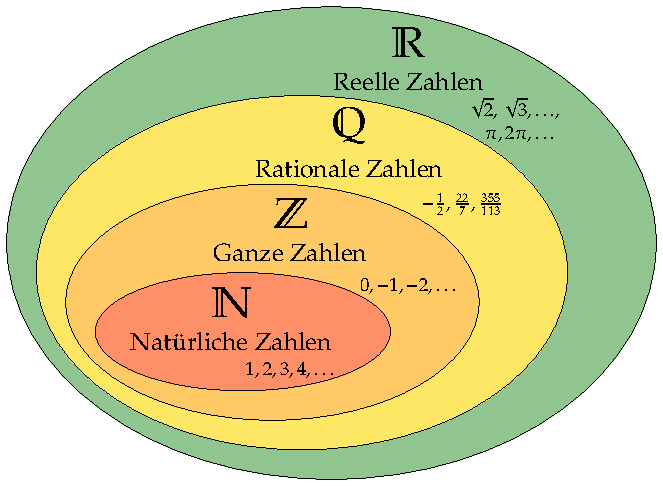
\includegraphics[width=\linewidth]{numberset-real}
	\vspace{-1cm}
\end{wrapfigure}
Da man $\sqrt{2}$ nicht als Bruch $\frac{p}{q}$ mit $p,q\in\Z$ darstellen kann, gilt:
\begin{align*}
  \sqrt{2} \notin \Q\, .
\end{align*}
Man nennt $\sqrt{2}$ eine sogenannte irrationale Zahl.
\begin{example}
 Kennst du bereits andere irrationale Zahlen? Welche?\\
 \kariert{7.5}{2}
\end{example}
\begin{example}
	Ist die Zahl rational oder irrational? Begründe.\\
	\begin{minipage}[t]{.3\linewidth}
		\begin{enumerate}[a)]
			\item $2.093903$
			\item $\frac{44}{45}$
		\end{enumerate}
	\end{minipage}
	\hfill
	\begin{minipage}[t]{.3\linewidth}
		\begin{enumerate}[a)]
		\setcounter{enumi}{2}
			\item $\sqrt{144}$
			\item $1.\overline{07}$
		\end{enumerate}
	\end{minipage}
	\hfill
	\begin{minipage}[t]{.3\linewidth}
		\begin{enumerate}[a)]
		\setcounter{enumi}{4}
			\item $1.090\,090\,009\,\ldots$
			\item $\sqrt{12}$
		\end{enumerate}
	\end{minipage}
	\vspace{.5cm}~\\
	{\bfseries Lösung:}
	\begin{enumerate}[a)]
        \setlength\itemsep{0pt}
        \item rational, da abbrechende Dezimalzahl und deshalb als Bruch darstellbar
        \item rational, da Bruch
        \item rational, da $\sqrt{144} = 12$
        \item rational, da periodische Dezimalzahl, siehe auch den Kasten auf Seite \pageref{law:periodicIsRational}.
        \item irrational, da weder abbrechende noch periodische Dezimalzahl
        \item irrational, da $\sqrt{12} = 2\cdot\sqrt{3}$\,.\\
        Angenommen, ~$2\cdot \sqrt{3}$ wäre doch rational. Zeige, dass daraus folgen würde, dass $\sqrt{3}$ rational ist.\\~\\
        \kariert{14}{3}\\~\\
        Dies ist ein Widerspruch dazu, dass $\sqrt{3}$ irrational ist.\\
        Also ist $\sqrt{12} = 2\cdot \sqrt{3}$ irrational.
    \end{enumerate}
\end{example}

Zusammenfassend können wir folgende Regeln festhalten:

\begin{law}{Regeln zum Erkennen von rationalen und irrationalen Zahlen}
	Ist eine Zahl z.B. eine
	\begin{itemize}\setlength\itemsep{0pt}
		\item abbrechende Dezimalzahl oder
		\item ein Bruch aus zwei ganzen Zahlen oder
		\item die Wurzel aus einer Quadratzahl oder
		\item eine periodische Dezimalzahl,
	\end{itemize}
	{\bfseries so ist sie eine rationale Zahl.}\\
	Ist sie hingegen
    \begin{itemize}\setlength\itemsep{0pt}
		\item eine Dezimalzahl, die weder abbricht, noch periodisch wird oder
		\item die Wurzel aus einer natürlichen Zahl, die keine Quadratzahl ist,
	\end{itemize}
	{\bfseries so ist sie eine irrationale Zahl.}
\end{law}

~\\
Zuammen bilden die Menge der rationalen Zahlen $\Q$ und die Menge der irrationalen Zahlen die Menge der sogenannten reellen Zahlen $\mathbb{R}$.
In dieser Menge, bzw. diesem Zahlenbereich gelten alle arithmetischen Rechengesetze von \pageref{law:arithmetic}.\\

\begin{defn}{Reelle Zahlen}
	Die Menge der reellen Zahlen $\R$ besteht aus allen rationalen und allen irrationen Zahlen.
	Es handelt sich um die Menge aller möglichen Zahlen, die man auf der Zahlengeraden darstellen kann.
\end{defn}

\subsection{Die Zahlengerade}
\begin{minipage}[t]{.5\linewidth}
 Erkläre anhand einer Zeichnung, wir man die Wurzel aus 2 auf der Zahlengerade darstellen kann:
\end{minipage}
\hfill
\begin{minipage}[t]{.45\linewidth}
~\\\vspace{-1.5cm}\\
 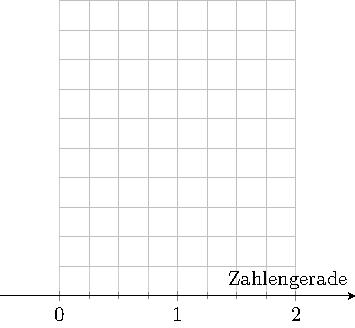
\includegraphics[width=\linewidth]{zahlengerade-Wurzel2}
\end{minipage}


\subsection{Für Interessierte: Gibt es Zahlen, die nicht reell sind?}
Bisher wurden die Erweiterungen der Zahlenbereiche dadurch begründet, dass uns (d.h. der Menschheit) der jeweils alte Zahlenbereich nicht ausgereicht hat, um bestimmte Gleichungen zu lösen.
Zum Beispiel konnten wir im Zahlenbereich der natürlichen Zahlen $\N$ die Gleichung $3 + x = 1$ nicht lösen.
Also haben wir die ganzen Zahlen $\Z$ eingeführt und konnten die Gleichung nun durch $x = -2$ lösen.

Dann hat uns z.B. die Lösung der Gleichung $3\cdot x = 1$ gefehlt -- also haben wir die rationalen Zahlen eingeführt und konnten nun $x = \frac{1}{3}$ setzen.
Als nächsten wollten wir die Gleichung $x^2 = 2$ lösen und haben festgestellt, dass uns hierzu wiederum die rationalen Zahlen nicht ausreichen.
Also haben wir unseren Zahlenbereich auf den Bereich der reellen Zahlen $\R$ erweitert und erhielten so die irrationale Zahl $\sqrt{2}$ als Lösung.
Hier waren wir aber nicht ganz konsequent, denn die Gleichung
\begin{align*}
	x^2 = -1
\end{align*}
können wir immer noch nicht lösen.
Egal, welche reelle Zahl wir für $x$ einsetzen, das Ergebnis von $x^2$ wird immer nicht nicht-negativ sein.

Um die obige Gleichung zu lösen, wurde ein neuer Zahlenbereich eingeführt -- der Zahlenbereich der komplexen Zahlen $\C$.
Dieser enthält u.a. die sogenannte \emph{imaginäre Einheit $\im$}, die genau so definiert ist, dass
\begin{align*}
	\im^2 = -1
\end{align*}
gilt.
Die Vielfachen von $\im$, wie z.B. $2\im, 3\im\, 4\im, \ldots$ nennen wir \emph{imaginäre Zahlen} und die Kombinationen $x + \im y$ mit $x$ und $y$ aus $\R$ nennen wir komplexe Zahlen, also z.B.:
\begin{align*}
	1 + \im \in \C;\qquad 2 - \im \in \C;\qquad 0.25 + 1.75\im \in \C \qquad \text{etc.}
\end{align*}

\begin{wrapfigure}{r}{.6\linewidth}
	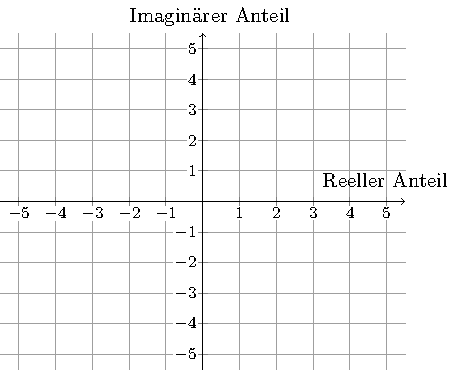
\includegraphics[width=\linewidth]{KomplexeEbene}
	\caption{Die komplexe Zahlenebene.}
	\label{fig:complexPlain}
\end{wrapfigure}
Zur grafischen Darstellung der komplexen Zahlen reicht uns die Zahlengerade nicht mehr aus.
Stattdessen verwenden wir die sogenannte \emph{komplexe Zahlenebene}, mit einem Koordinatensystem, dessen $x$-Achse die reellen Zahlen darstellt und dessen $y$-Achse die imaginären, siehe Abbildung \ref{fig:complexPlain}.
Die komplexe Zahl $1 + \im$ entspricht dann einem Punkt mit den Koordinaten $(1\,|\,1)$, die komplexe Zahl $2 - \im$ entspricht dem Punkt $(2\,|\,-1)$.

\section{Mächtigkeit (Kardinalität) der Zahlenmengen}
Oftmals enthalten Mengen eine endliche Anzahl Elemente, d.h., man kann genau angeben, wieviele es sind. Bei den Zahlenmengen ist das etwas schwieriger. Es gibt unendlich viele natürliche Zahlen. Es gibt aber auch unendlich viele reelle Zahlen. Gibt es also gleich viele von beiden? Diese Fragen wollen wir nun beantworten.

\subsection{Mächtigkeit}
Die Menge $M$ der Mitgliedstaaten der EU unfasst 27 Länder.\\
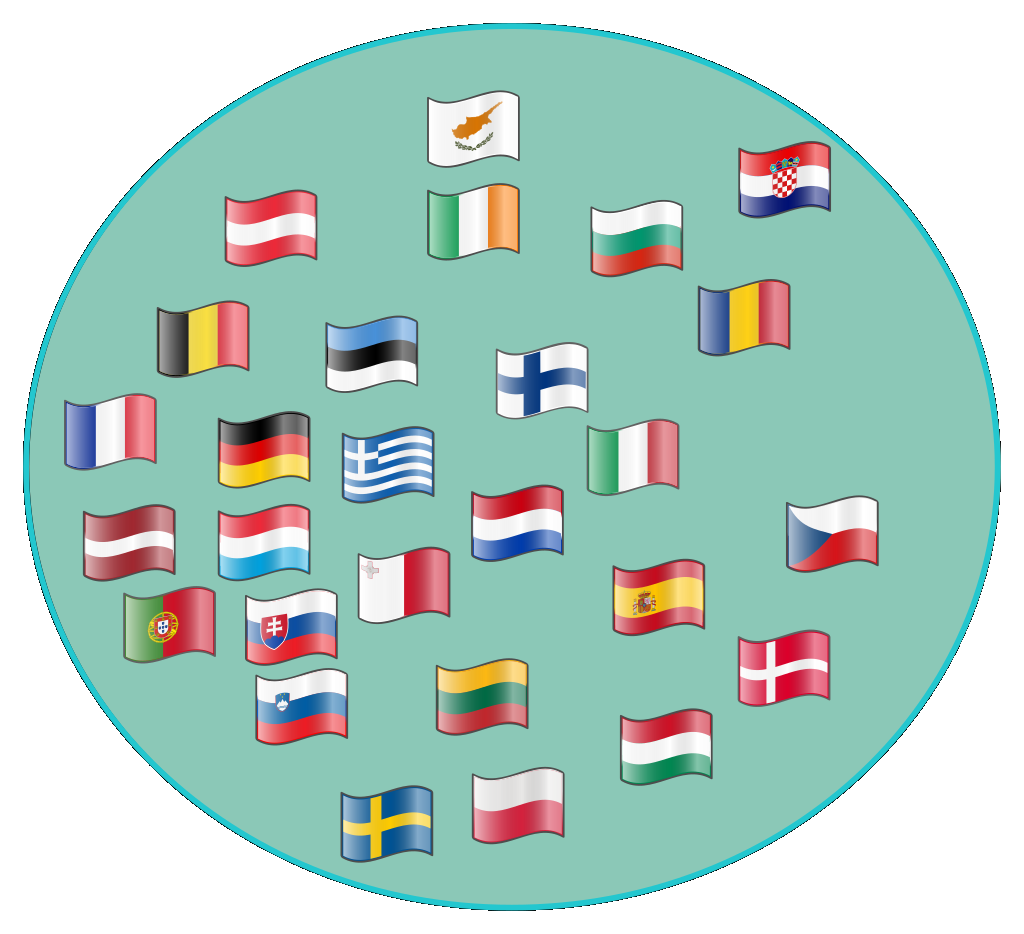
\includegraphics[width=0.4\linewidth]{EU-Mitgliedstaaten}

Man kann diese Menge aber auch in aufzählender Form angeben:\\
\emph{M} = $\{$Belgien, Bulgarien, Dänemark, Deutschland, Estland, Finnland, Frankreich,\\ Griechenland, Irland, Italien, Kroatien, Lettland, Litauen, Luxemburg,\\ Malta, Niederlande, Österreich, Polen, Portugal, Rumänien, Schweden,\\ Slowakei, Slowenien, Spanien, Tschechien, Ungarn, Zypern$\}$

Das sind 27 Länder. Man sagt: "`Die \textbf{Mächtigkeit} oder \textbf{Kardinalität} der Menge $M$ ist 27"', oder: $|M|=27$

\begin{defn}{Mächtigkeit (Kardinalität) einer Menge}
	Für endliche Mengen ist die Mächtigkeit gleich der Anzahl der Elemente der Menge, das ist eine natürliche Zahl einschließlich der Null. 
\end{defn}~
\vspace{5mm}


\begin{example}
	Weitere Beispiele sind:
	\begin{enumerate}
		\item
			$A=\{1, 3, 7 21\}$, \quad $|A|=4$
		\item
			$B=\{\textrm{Tetraeder, Hexaeder, Oktaeder, Dodekaeder, Ikosaeder}\}$, \quad $|B|=5$
		\item
			$C=\{\textrm{rot, gelb, blau, orange, violett, schwarz}\}$, \quad $|C|=6$
	\end{enumerate}
\end{example}

Mit Zahlenmengen wird das schwierig oder unübersichtlich. Schauen wir die natürlichen Zahlen an, können wir diese angeben als

\vspace{1.5cm}

Geht das auch mit den rationalen Zahlen? Und mit den reellen Zahlen? Versuche es!

\vspace{1.5cm}

Es braucht also etwas Vorarbeit, um die Mächtigeit dieser Zahlenmengen zu charakterisieren. Dabei werden wir zum ersten Mal einem wichtigen Begriff begegnen: Der Unendlichkeit! 

\begin{task}{Auftrag}
Wir schauen uns gemeinsam ein Video zu diesem Thema an. Mach dir Notizen zu den wichtigsten Aussagen! Anschliessend diskutiert ihr zu zweit die folgenden Fragen:
	\begin{itemize}
		\item
			Wann kann man sagen, dass zwei Mengen gleich mächtig sind?
		\item
			Wie hat Georg Cantor gezeigt, dass die natürlichen Zahlen gleich mächtig sind wie die rationalen?
		\item
			Wie lässt sich argumentieren, dass dir reellen Zahlen mächtiger sind, als die natürlichen und dir rationalen?
	\end{itemize}
	Bei der Beantwortung der Fragen sollt ihr die untenstehenden Diagramm verwenden: Welche Aussage steht jeweils mit dem Diagramm in Verbindung? Und falls ihr eine Szene des Films nochmal anschauen wollt, könnt ihr ihn mit eurem Notebook oder Smartphone noch einmal aufrufen:\\
	
\includegraphics{QR-Video-Kardinalitaet-HS24}
\end{task}

Los geht's auf der nächsten Seite!

\newpage

\fbox{\parbox{\linewidth}{
\emph{Meinen Notizen zum Film:}\par \vspace*{7cm}}}

\subsection{Bijektion}
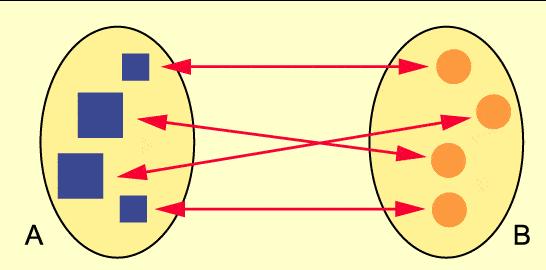
\includegraphics[width=.4\linewidth]{Bijektion}

\subsection{Mächtigkeit der rationalen Zahlen}
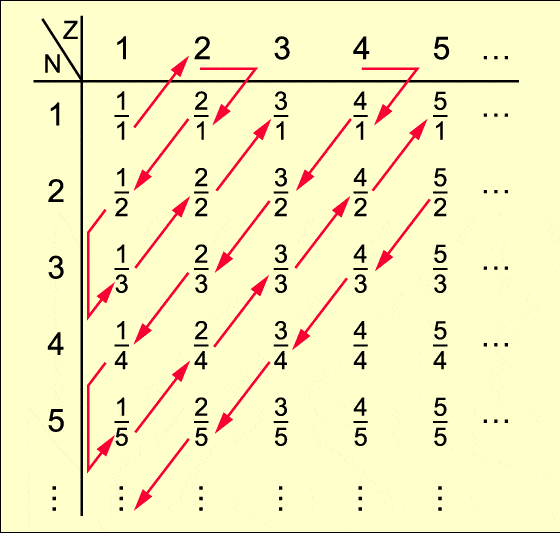
\includegraphics[width=.4\linewidth]{RationaleZahlen}

\subsection{Mächtigkeit der reellen Zahlen}
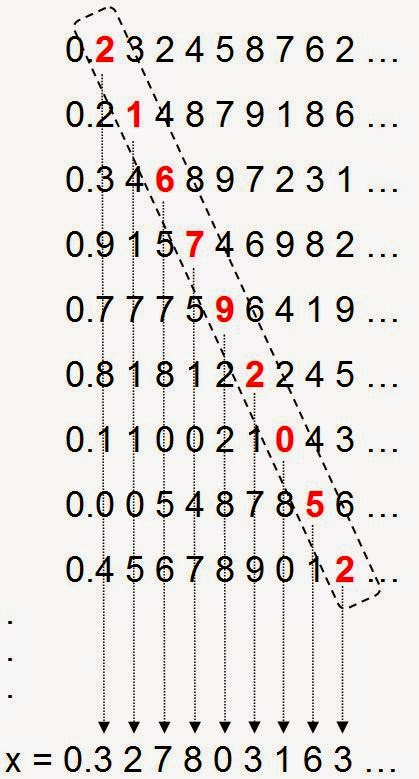
\includegraphics[width=.4\linewidth]{Cantor-diagonal-2}

\newpage

\section{Andere Zahlsysteme}
Das verbreitete, von uns benutzte Dezimalsystem ist nur eine Möglichkeit, Zahlen zu beschreiben. Computer z.B. benutzen das Binärsystem.

\subsection*{Das Dezimalsystem}
Wir sind es gewohnt, Berechnungen im Dezimalsystem durchzuführen, in dem jede Zahl einer bestimmten Zusammensetzung der zehn verschiedenen Ziffern 0, 1, 2, 3, 4, 5, 6, 7, 8, 9 entspricht. Jede Stelle \emph{vor} dem Komma (oder dem Dezimalpunkt) repräsentiert ein Vielfaches von 0 bis 9 der Potenzen von 10 mit positivem, ganzzahligem Exponenten (inklusive 0), und jede Stelle \emph{hinter} dem Komma repräsentiert ein Vielfaches von 0 bis 9 der \vspace{.6cm} \\ \vspace{.6cm} .\dotfill{}. \\  .\dotfill{}.

\begin{example}[Zahlen im Dezimalsystem]\hfill
    \begin{enumerate}
        \item $\textbf{31} = 3 \cdot 10 + 1 = \textbf{3} \cdot 10^1 + \textbf{1} \cdot 10^0$
        \item $2357 = 2 \cdot 1000 + 3 \cdot 100 + 5 \cdot 10 + 7 = 2 \cdot 10^3 + 3 \cdot 10^2 + 5 \cdot 10^1 + 7 \cdot 10^0$
        \item $250.71 = 2 \cdot 100 + 5 \cdot 10 + 0 + 7 \cdot 0.1 + 1 \cdot 0.01 = 2 \cdot 10^2 + 5 \cdot 10^1 + 0 \cdot 10^0 + 7 \cdot 10^{-1} + 1 \cdot 10^{-2}$
        \item $98437=$
        \item $0.00321=$
    \end{enumerate}
\end{example}

\subsection*{Das Binärsystem}
Benutzen wir 2 anstatt 10 als Basis, erhalten wir das sogenannte binäre Zahlensystem, oder kurz Binärsystem. Die Ziffern im Binärsystem sind 1 und 0. Die Stellen einer Zahl im Binärsystem entsprechen Vielfachen von 0 bis 1 der Potenzen von 2.

\begin{example}[Zahlen im Binärsystem]\hfill
    \begin{enumerate}
        \item $\textbf{110} = \textbf{1} \cdot 2^2 + \textbf{1} \cdot 2^1 + \textbf{0} \cdot 2^0 = 4 + 2 = 6$
        \item $100110 = 1 \cdot 2^5 + 0 \cdot 2^4 + 0 \cdot 2^3 + 1 \cdot 2^2 + 1 \cdot 2^1 + 0 \cdot 2^0 = 32 + 4 + 2 = 38$
        \item $11001001 = $
    \end{enumerate}
\end{example}


\subsubsection*{Zählen mit den Fingern}

\begin{minipage}{.5\textwidth}
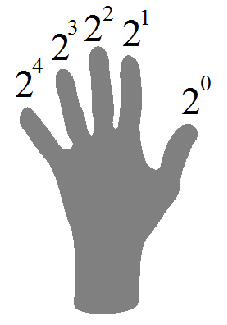
\includegraphics[width=0.5\linewidth]{BinaryHand}
\end{minipage}
\hspace*{.1\textwidth}
\begin{minipage}{.4\textwidth}
Man kann auch im Binärsystem mit den Fingern zählen. Dabei entspricht jeder Finger einer Zweierpotenz.
    \begin{tabular}{clcl}
        $\bullet$ & Finger oben & $\longrightarrow$ & \textbf{1} \\
        $\bullet$ & Finger unten & $\longrightarrow$ & \textbf{0}
    \end{tabular}
\end{minipage}

\begin{example} $ $ \\
\begin{minipage}{.3\textwidth}
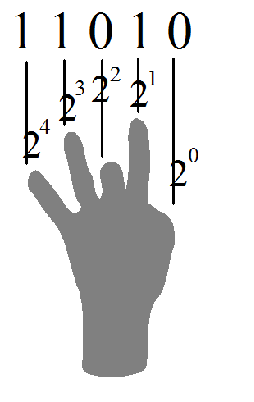
\includegraphics[width=\linewidth]{BinaryHand2}
\end{minipage}
\hspace*{.1\textwidth}
\begin{minipage}{.6\textwidth}
Schauen wir uns beispielsweise diese Hand an:

\hspace{.5cm}

    \begin{tabular}{lcccccl}
        Finger & Kleiner & Ring- & Mittel- & Zeige- & Daumen \\
        Position & oben & oben & unten & oben & unten \\
        Stele & 1 & 1 & 0 & 1 & 0 \\
        Potenz & $2^4$ & $2^3$ & $2^2$ & $2^1$ & $2^0$ \\
        Wert & 16 & 8 & 0 & 2 & 0 \\
    \end{tabular}

\hspace{.5cm}

Wir wir alle Werte zusammenzählen, bekommen wir --- auf den Fingern einer Hand! Wie weit kann man mit beiden Händen zählen?
\end{minipage}

\end{example}

\begin{exercise}
	Übersetze ins angegebene Dezimalsystem:
	\begin{enumerate}
		\item
			Übersetze ins Dezimalsystem: $10011100_{2}$
		\item
			Übersetze ins Binärsystem: $825_{10}$
	\end{enumerate}
\end{exercise}

\newpage

\subsection{Für Interessierte\ldots}
Es gibt natürlich noch weitere Zahlensysteme. Als Basis könnten wir z.B. auch die 3 oder die 16 wählen.

\subsubsection{Das Ternärsystem}
Das System mit der Basis 3 heisst - analog zum Binärsystem mit der Basis 2 - Ternärsystem. Jedes Zahlsystem benötigt soviele Ziffern, wie der Wert der Basis ist. Es sind jeweils die Ziffern bis eine vor dem Basiswert, beginnend mit der Null. Das Binärsystem mit der Basis 2 benötigt zwei Ziffern, 0 und 1, das Dezimalsystem hat zehn Ziffern, nämlich 0, 1, 2, 3, 4, 5, 6, 7, 8, 9, und das Ternärsystem entsprechend drei: 0, 1, 2.

\begin{example}
	Die Ziffern werden mit den Potenzen von 3 multipliziert.\\
	$\textbf{201\textsubscript{3}} = \textbf{2} \cdot 3^2 + \textbf{0} \cdot 3^1 + \textbf{1} \cdot 3^0 = 9 + 1 = 10$
\end{example}

\begin{exercise}
	Übersetze ins Dezimalsystem: $12021_{3}$
	\vfill
\end{exercise}

\begin{minipage}[t]{.5\linewidth}
	Es gab sogar mal einen Computer, der an der Universität Moskau entwickelt worden war und anstatt mit dem binären mit dem ternären System arbeitete! Anstatt Bits hatte dieser Computer Trits, und Bytes waren Trytes. Er hatte aber keine Vorteile gegenüber der damals bereits weit entwickelten binären Technologie, und wurd daher ab den 1970er-Jahren nicht mehr weiterentwickelt.
\end{minipage}
\hspace{.1\linewidth}
\begin{minipage}[t]{.4\linewidth}
	\vspace{-\ht\strutbox}
	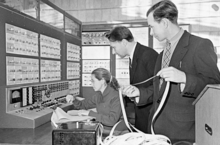
\includegraphics{Setun}
\end{minipage}


\subsubsection{Das Hexadezimalsystem}
Das Hexadezimalsystem\footnote{\emph{Hexadezimal} ist ein griechisch-lateinisches Mischwort aus griech. \emph{hexa} für sechs und lat. \emph{decem} für zehn.} hat die Basis 16 und wird noch heute in der Informatik verwendet. Sein Nutzen liegt darin, dass 16 die vierte Potenz von 2 ist und damit ein Byte (= 8 Bits\footnote{\textbf{B}inary dig\textbf{its}, also Binärziffern}) mit nur einer Ziffer des Hexadezimalsystems dargestellt werden kann. Oftmals werden zum Beispiel Farben des \textcolor{red}{R}\textcolor{green}{G}\textcolor{blue}{B}-Systems am Computer mit diesem System codiert. Zur Basis 16 benötigen wir sechzehn Ziffern - aber halt, da reichen ja die Ziffern 0 bis 9 nicht mehr aus! Genau. Deshalb nehmen wir einfach noch die Buchstaben A, B, C, D, E, und F dazu. Dann entsprechen

\begin{table}[H]
	\caption{Bedeutung der "`Buchstaben-Ziffern"' im Hexadezimalsystem}
	\centering
	\begin{tabular}{|c|c|}
		\hline
		A & 10 \\
		B & 11 \\
		C & 12 \\
		D & 13 \\
		E & 14 \\
		F & 15 \\
		\hline
	\end{tabular}
\end{table}

\begin{example}
		$\textbf{2C7\textsubscript{16}} = \textbf{2} \cdot 16^2 + \textbf{12} \cdot 16^1 + \textbf{7} \cdot 16^0 = 256 + 192 + 1 = 455 $
\end{example}

Figur \ref{fig:Farbcodierung} zeigt, wie diese Codierung dann aussieht.

\begin{figure}[h]
	\centering
	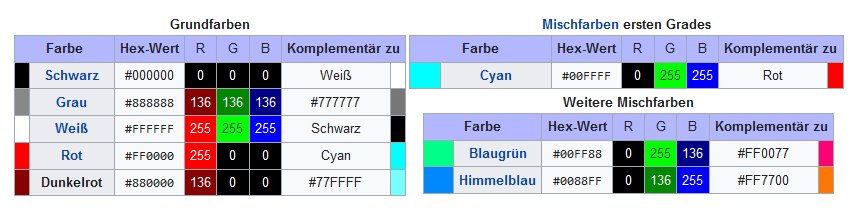
\includegraphics[width=\linewidth]{Farbcodierung}
	\caption{Die Codierung von RGB-Farben am Computer mit dem Hexadezimalsystem. (Quelle: Wikipedia)}
	\label{fig:Farbcodierung}
\end{figure}

Grundlage dafür ist die additive Farbmischung (Videolink zum Thema am Rand) Üblich ist die Darstellung als Aneinanderreihung von drei jeweils zweistellig geschriebenen Hexadezimalzahlen nach dem Muster: \#\textcolor{red}{RR}\textcolor{green}{GG}\textcolor{blue}{BB}. Dabei steht der Wert 0 für eine komplett abgedunkelte = ausgeschaltete Farbesgeschaltete“ und 255 (FF) für volle Farbsättigung. Der Code \#FFFF00 ergibt Beispielsweise die Farbe Gelb, weil Rot (\#FF0000) mit Grün (\#00FF00) gemischt wird. Diese Art der Notation wird häufig für Webfarben zur farblichen Gestaltung von Internetseiten verwendet. \marginpar{
\includegraphics{QR-Video-Additive-Farbmischung}}


\section{Mengenrelationen}
Wenn wir von Zahlenmengen und Mengen in einem viel allgemeineren Kontext sprechen, so können wir auch noch Beziehung von Mengen untereinander Darstellen. Zum Beispiel gehört die Menge der geraden Zahlen $P$ zu den natürlichen Zahlen, sie ist eine sogenannte Teilmenge davon. Diesen Begriffen wollen wir noch auf die Spur kommen.

\subsection{Mengendiagramme (Venndiagramme)}
Die Beziehungen zwischen 2 oder 3 Mengen stellen wir grafisch in sogenannten Venndiagrammen dar. Es sind Mengendiagramme, die man zu Ehren ihres Erfinders, John Venn, so benannt hat. Betrachten wir zum Beispiel die drei folgenden Mengen:
\begin{align*}
	A &= \{1,3,5,10,15\} \\
	B &= \{1,5,10\} \\
	C &= \{3, 15, 16 \}
\end{align*}

Die Mengen $A$ und $B$ haben einige Elemente gemeinsam, aber nicht alle, ebenso $A$ und $C$, aber $B$ und $C$ haben keine gemeinsamen Elemente. Grafisch wird das viel übersichtlicher:

\begin{figure}[H]
	\centering
	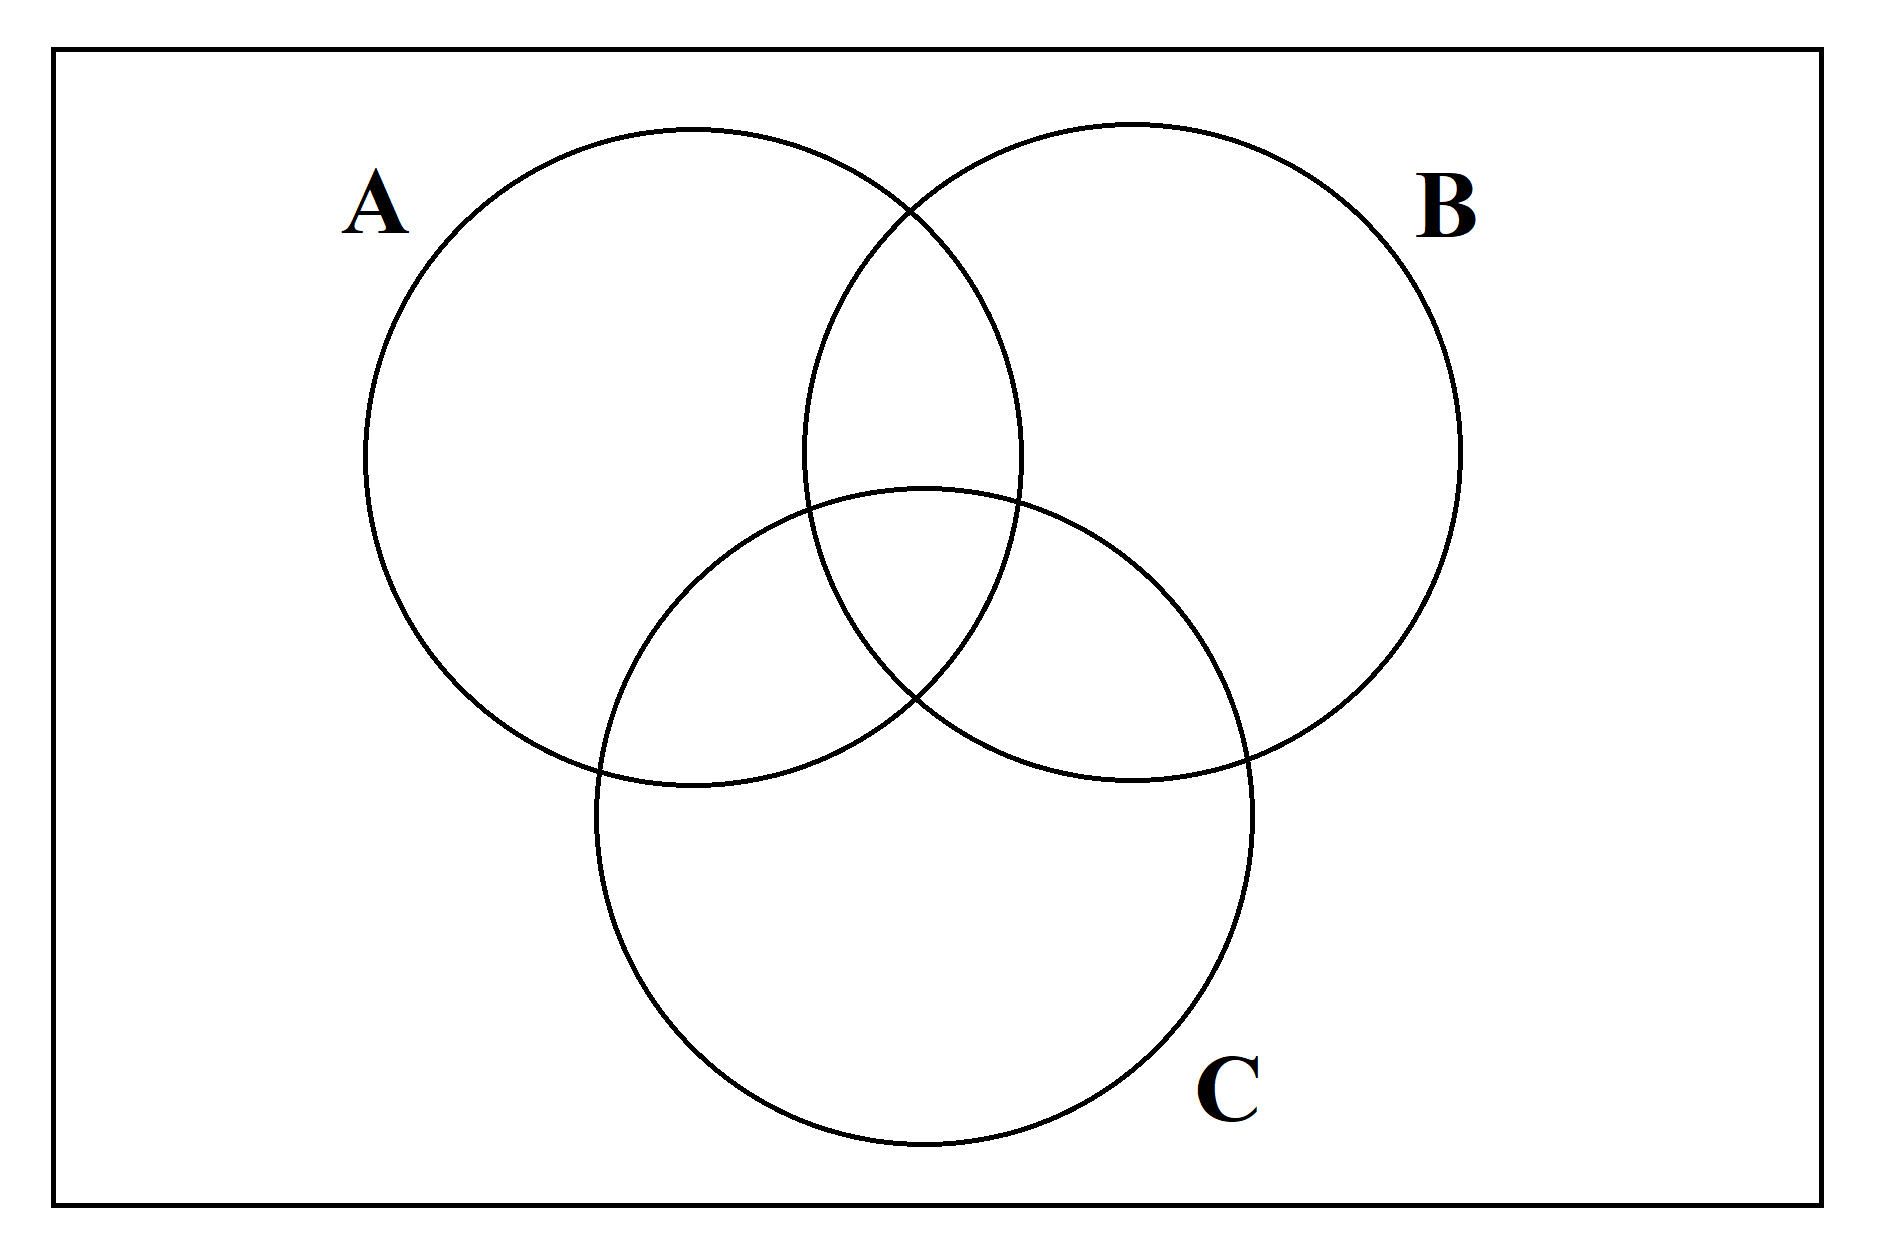
\includegraphics[width=.8\linewidth]{Venndiagramm}
	\caption{Darstellung in einem Venndiagramm}
\end{figure}

Dafür können wir auch eine Symbolsprache einführen:

\begin{law}{Mengenrelationen}
	\begin{tabular}{r @{\hspace{5mm}:\hspace{5mm}} l}
		$\subset$ & ist Teilmenge von \\
		$\not\subset$ & ist keine Teilmenge von \\
		$\backslash$ & ohne \\
		$\cap$ & geschnitten mit \\
		$\cup$ & vereinigt mit
	\end{tabular}
\end{law}

\begin{exercise}
	Ordne den folgenden Bildern die richtige Relation zu!
	\vspace{3cm}
	\begin{figure}[H]
		\centering
		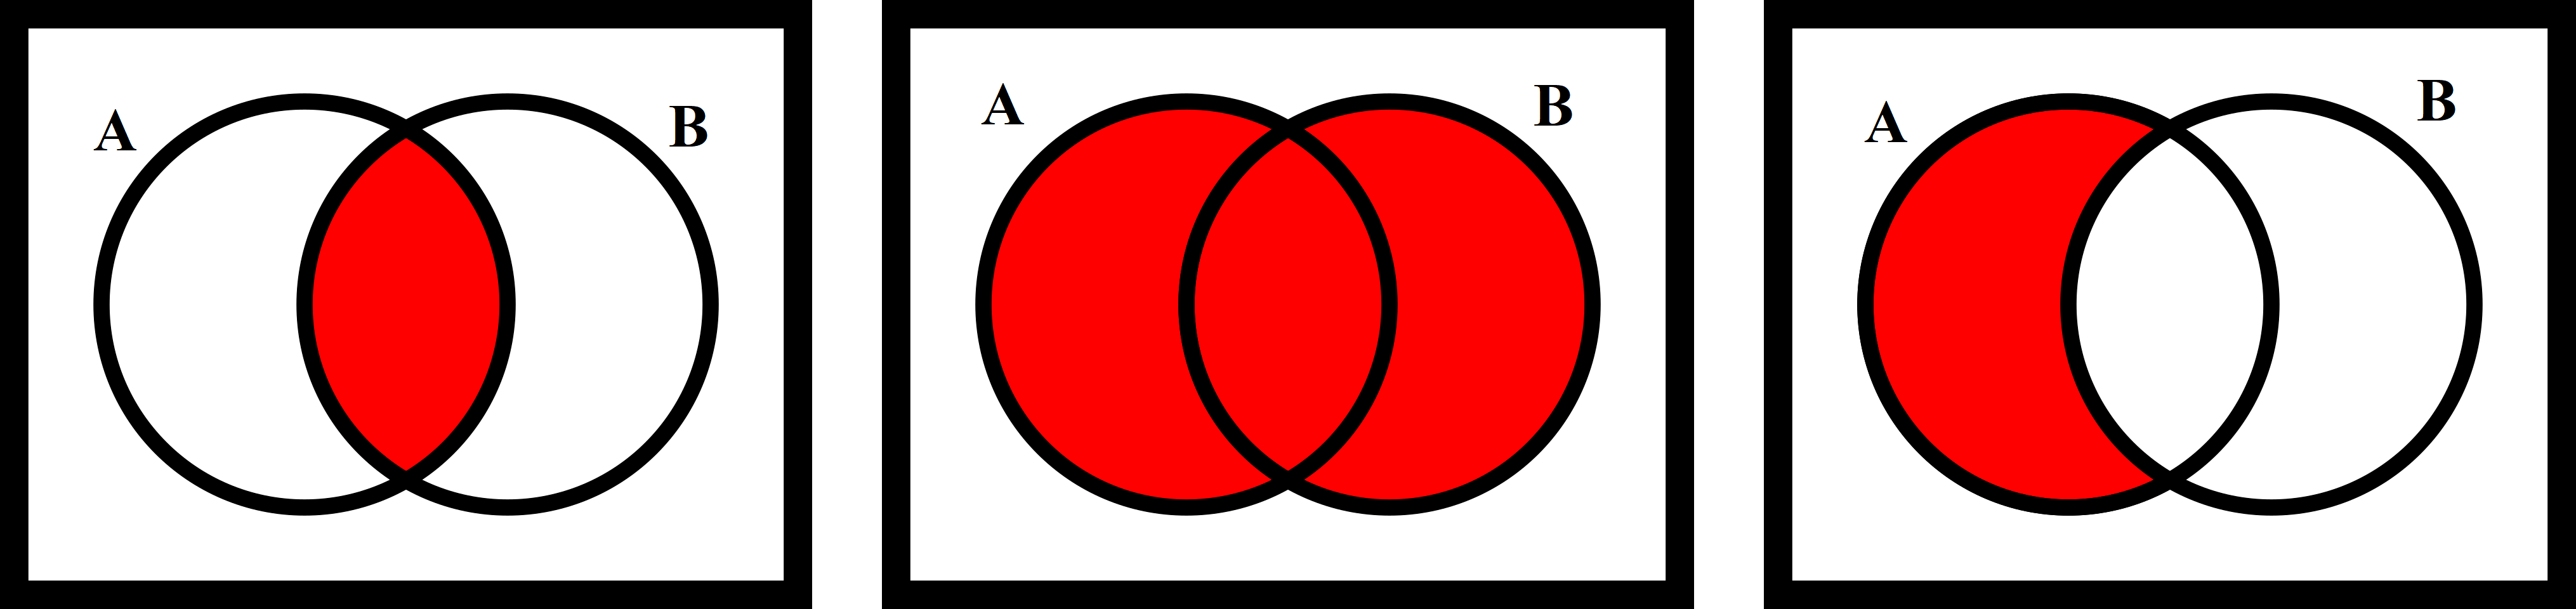
\includegraphics[width=.8\linewidth]{Venndiagramme}
		\caption{Spezielle Relationen zwischen Mengen, dargestellt mit Venndiagrammen}
	\end{figure}
\end{exercise}

Zeit für ein paar Übungsaufgaben!

\paragraph{Aufgaben im Buch, Seite 17}
$ $ \newline
\begin{tabular}{|lll|}
\hline
\textbf{Grundlagen} & \textbf{Training} & \textbf{Extra}\\
\hline
117-123 & & \\
\hline
\end{tabular}

\newpage

% \section{Rechnen mit Potenzen}
% Positive und negative Exponenten, Potenzgesetze, Zehnerpotenzen und wissenschaftliche Schreibweise, viele Übungen
% 
% Am Schluss: $(a+b)^n \ne a^n+b^n$
